\documentclass[12pt,a4paper,openany]{book}
\usepackage{lmodern}
\usepackage[table]{xcolor}
\usepackage{xcolor}
\definecolor{vert1}{rgb}{0.0,0.3.9,0.0}
\definecolor{bleu}{rgb}{0,0,0.5}
\definecolor{bleu3}{rgb}{1,0.2,0.2}
\definecolor{grisgris}{gray}{0.4}
\definecolor{rougeUPS}{rgb}{0.6, 0.3, 0.3}

\fboxsep =0pt \parindent =0pt\parskip =12pt



\usepackage[utf8]{inputenc} \usepackage[T1]{fontenc}
\usepackage{pdfpages}
\usepackage[francais]{babel}
\usepackage[top=1.7cm, bottom=1.7cm, left=1.7cm, right=1.7cm]{geometry}
\usepackage{verbatim}
\usepackage[urlbordercolor={1 1 1}, linkbordercolor={1 1 1}, linkcolor=vert1, urlcolor=bleu, colorlinks=true]{hyperref}
\usepackage{tikz} %Vectoriel
\usepackage{listings}
\usepackage{fancyhdr}
\usepackage{multido}
\usepackage{float}
\usepackage{amssymb}

\newcommand{\titre}{Dossier final}

\newcommand{\pole}{}
\newcommand{\sigle}{}

\newcommand{\semestre}{4}

\definecolor{gris1}{gray}{0.40}
\definecolor{gris2}{gray}{0.55}
\definecolor{gris3}{gray}{0.65}
\definecolor{gris4}{gray}{0.50}
\definecolor{vert}{rgb}{0,0.4,0}
\definecolor{violet}{rgb}{0.65, 0.2, 0.65}
\definecolor{bleu1}{rgb}{0,0,0.8}
\definecolor{bleu2}{rgb}{0,0.2,0.6}
\definecolor{bleu3}{rgb}{0,0.2,0.2}
\definecolor{rouge}{HTML}{F93928}


\lstdefinelanguage{algo}{%
   morekeywords={%
    %%% couleur 1
		importer, programme, glossaire, fonction, procedure, constante, type, 
	%%% IMPORT & Co.
		si, sinon, alors, fin, tantque, debut, faire, lorsque, fin lorsque, 
		declenche, declencher, enregistrement, tableau, retourne, retourner, =, pour, a,
		/=, <, >, traite,exception, 
	%%% types 
		Entier, Reel, Booleen, Caractere, Réél, Booléen, Caractère,
	%%% types 
		entree, maj, sortie,entrée,
	%%% types 
		et, ou, non,
	},
  sensitive=true,
  morecomment=[l]{--},
  morestring=[b]',
}

\lstset{language=algo,
    %%% BOUCLE, TEST & Co.
      emph={importer, programme, glossaire, fonction, procedure, constante, type},
      emphstyle=\color{bleu2},
    %%% IMPORT & Co.  
	emph={[2]
		si, sinon, alors, fin , tantque, debut, faire, lorsque, fin lorsque, 
		declencher, retourner, et, ou, non,enregistrement, retourner, retourne, 
		tableau, /=, <, =, >, traite,exception, pour, a
	},
      emphstyle=[2]\color{bleu1},
    %%% FONCTIONS NUMERIQUES
      emph={[3]Entier, Reel, Booleen, Caractere, Booléen, Réél, Caractère},
      emphstyle=[3]\color{gris1},
    %%% FONCTIONS NUMERIQUES
      emph={[4]entree, maj, sortie, entrée},	
      emphstyle=[4]\color{gris1},
}
\lstdefinelanguage{wl}{%
   morekeywords={%
    %%% couleur 1
		importer, programme, glossaire, fonction, procedure, constante, type, 
	%%% IMPORT & Co.
		si, sinon, alors, fin, TANTQUE, tantque, FIN, PROCEDURE, debut, faire, lorsque, 
		fin lorsque, declenche, declencher, enregistrement, tableau, retourne, retourner, =, 
		/=, <, >, traite,exception, 
	%%% types 
		Entier, Reel, Booleen, Caractere, Réél, Booléen, Caractère,
	%%% types 
		entree, maj, sortie,entrée,
	%%% types 
		et, ou, non,
	},
  sensitive=true,
  morecomment=[l]{//},
  morestring=[b]',
}

\lstset{language=wl,
    %%% BOUCLE, TEST & Co.
      emph={importer, programme, glossaire, fonction, procedure, constante, type},
      emphstyle=\color{bleu2},
    %%% IMPORT & Co.  
	emph={[2]
		si, sinon, alors, fin , tantque, debut, faire, lorsque, fin lorsque, 
		declencher, retourner, et, ou, non,enregistrement, retourner, retourne, 
		tableau, /=, <, =, >, traite,exception
	},
      emphstyle=[2]\color{bleu1},
    %%% FONCTIONS NUMERIQUES
      emph={[3]Entier, Reel, Booleen, Caractere, Booléen, Réél, Caractère},
      emphstyle=[3]\color{gris1},
    %%% FONCTIONS NUMERIQUES
      emph={[4]entree, maj, sortie, entrée},	
      emphstyle=[4]\color{gris1},
}
\lstdefinelanguage{css}{%
   morekeywords={%
    %%% couleur 1
		background, image, repeat, position, index, color, border, font, 
		size, url, family, style, variant, weight, letter, spacing, line, 
		height, text, decoration, align, indent, transform, shadow, 
		background, image, repeat, position, index, color, border, font, 
		size, url, family, style, variant, weight, letter, spacing, line, 
		height, text, decoration, align, indent, transform, shadow, 
		vertical, align, white, space, word, spacing,attachment, width, 
		max, min, margin, padding, clip, direction, display, overflow,
		visibility, clear, float, top, right, bottom, left, list, type, 
		collapse, side, empty, cells, table, layout, cursor, marks, page, break,
		before, after, inside, orphans, windows, azimuth, after, before, cue, 
		elevation, pause, play, during, pitch, range, richness, spek, header, 
		numeral, punctuation, rate, stress, voice, volume,
	%%% types 
		left, right, bottom, top, none, center, solid, black, blue, red, green,
	},
  sensitive=true,
  sensitive=true,
  morecomment=[s]{/*}{*/},
  morestring=[b]',
}
\lstset{language=css,
    %%% BOUCLE, TEST & Co.
      emph={
		background, image, repeat, position, index, color, border, font, 
		size, url, family, style, variant, weight, letter, spacing, line, 
		height, text, decoration, align, indent, transform, shadow, 
		background, image, repeat, position, index, color, border, font, 
		size, url, family, style, variant, weight, letter, spacing, line, 
		height, text, decoration, align, indent, transform, shadow, 
		vertical, align, white, space, word, spacing,attachment, width, 
		max, min, margin, padding, clip, direction, display, overflow,
		visibility, clear, float, top, right, bottom, left, list, type, 
		collapse, side, empty, cells, table, layout, cursor, marks, page, break,
		before, after, inside, orphans, windows, azimuth, after, before, cue, 
		elevation, pause, play, during, pitch, range, richness, spek, header, 
		numeral, punctuation, rate, stress, voice, volume,
	  },
      emphstyle=\color{bleu2},
    %%% FONCTIONS NUMERIQUES
      emph={[3]
		left, right, bottom, top,none, solid, black, blue, green,
		  },
      emphstyle=[3]\color{bleu3},
    %%% FONCTIONS NUMERIQUES
}

\lstset{language=SQL,
    %%% BOUCLE, TEST & Co.
      emph={INSERT, UPDATE, DELETE, WHERE, SET, GROUP, BY, ORDER},
      emphstyle=\color{bleu2},
    %%% IMPORT & Co.  
	emph={[2]
		if, end, begin, then, for, each, else, after, of, on, to
	},
      emphstyle=[2]\color{bleu1},
    %%% FONCTIONS NUMERIQUES
      emph={[3]Entier, Reel, Booleen, Caractere, Booléen, Réél, Caractère},
      emphstyle=[3]\color{gris1},
    %%% FONCTIONS NUMERIQUES
      emph={[4]entree, maj, sortie, entrée},	
      emphstyle=[4]\color{gris1},
}
\lstdefinelanguage{ARM}{%
   morekeywords={%
   ADD, SUB, MOV, MUL, RSB,CMP, BLS, BLE, B,BHI,
   BGE, RSBLT, BGT, BEQ, BNE,BLT
	},
  sensitive=true,
  morecomment=[l]{@},
  morestring=[b]',
}

\lstset{ % general style for listings 
   numbers=left 
   , literate={é}{{\'e}}1 {è}{{\`e}}1 {à}{{\`a}}1 {ê}{{\^e}}1 {É}{{\'E}}1 {ô}{{\^o}}1 {€}{{\euro}}1{°}{{$^{\circ}$}}1 {ç}{ {c}}1
	, extendedchars=\true
   , tabsize=2 
   , frame=l
   , framerule=1.1pt
   , linewidth=520px
   , breaklines=true 
   , basicstyle=\footnotesize\ttfamily 
   , numberstyle=\tiny\ttfamily 
   , framexleftmargin=0mm 
   , xleftmargin=0mm 
   , captionpos=b 
	, keywordstyle=\color{bleu2}
	, commentstyle=\color{vert}
	, stringstyle=\color{rouge}
	, showstringspaces=false
	, extendedchars=true
	, mathescape=true
} 
%	\lstlistoflistings
%	\addcontentsline{toc}{part}{List of code examples}

%\date{\today}

\makeindex
\lfoot{Université Toulouse III -- Paul Sabatier}
\rfoot{}
%\rfoot{}
\cfoot{}
\makeglossary
\makeatletter
\def\clap#1{\hbox to 0pt{\hss #1\hss}}%
\def\ligne#1{%
\hbox to \hsize{%
\vbox{\centering #1}}}%
\def\haut#1#2#3{%
\hbox to \hsize{%
\rlap{\vtop{\raggedright #1}}%
\hss
\clap{\vtop{\centering #2}}%
\hss
\llap{\vtop{\raggedleft #3}}}}%
\def\bas#1#2#3{%
\hbox to \hsize{%
\rlap{\vbox{\raggedright #1}}%
\hss \clap{\vbox{\centering #2}}%
\hss
\llap{\vbox{\raggedleft #3}}}}%
\def\maketitle{%
\thispagestyle{empty}\vbox to \vsize{%
\haut{}{\@blurb}{}

\vfill
\vspace{1cm}
\begin{flushleft}
\usefont{OT1}{ptm}{m}{n}
\huge \@title
\end{flushleft}
\par
\hrule height 4pt
\par
\begin{flushright}
\usefont{OT1}{phv}{m}{n}
\Large \@author
\par
\end{flushright}
\vspace{1cm}
\vfill
\vfill
\bas{}{\@location, le \@date}{}
}%
\cleardoublepage
}
\def\date#1{\def\@date{#1}}
\def\author#1{\def\@author{#1}}
\def\title#1{\def\@title{#1}}
\def\location#1{\def\@location{#1}}
\def\blurb#1{\def\@blurb{#1}}
\date{\today}
\author{}
\title{}
\location{Amiens}\blurb{}
\makeatother
\title{\titre}
\author{Projet de Boggle}

\location{Toulouse}
\blurb{%
Université Toulouse III -- Paul sabatier\\
L2 Informatique\\
Projet tuteuré\\
\vspace{30px}
\begin{flushleft}Antoine de \bsc{Roquemaurel}\\ Fabrice
	\bsc{Valleix}\\ Groupe 2.2\end{flushleft}
}%



%\title{Cours \\ \titre}
%\date{\today\\ Semestre \semestre}

%\lhead{Cours: \titre}
%\chead{}
%\rhead{\thepage}

%\lfoot{Université Paul Sabatier Toulouse III}
%\cfoot{\thepage}
%\rfoot{\sigle\semestre}

\pagestyle{fancy}
%\renewcommand{\chaptermark}[1]{\markboth{\bsc{\chaptername~\thechapter{} :} #1}{}}
\renewcommand{\sectionmark}[1]{\markright{\thesection{ #1}}}
\renewcommand{\headrulewidth}{0.3pt}
\renewcommand{\footrulewidth}{0.3pt}

\fancyhf{}
\fancyhead[LO]{Antoine de \bsc{Roquemaurel} -- Fabrice \bsc{Valleix}}
\fancyhead[RO]{\rightmark}
\fancyfoot[CO]{--~\thepage~--}
\fancyfoot[LO]{Dossier de spécifications}
\fancyfoot[RO]{Projet de Boggle}
\fancyfoot[RE]{Antoine de \bsc{Roquemaurel} -- Fabrice \bsc{Valleix}}

%% Cas des premières pages de chapitre
\fancypagestyle{plain}{%
	\fancyhf{}%
	\fancyfoot[L]{\titre{}}
	\fancyfoot[R]{--~\thepage~--}
	\renewcommand{\headrulewidth}{0pt}
	\renewcommand{\footrulewidth}{0.3pt}
}
\makeatletter
\renewcommand*{\lstlistlistingname}{Liste des codes sources}
\renewcommand{\listfigurename}{Liste des figures}
\renewcommand\listoffigures{%
    \subsection{\listfigurename}%
      \@mkboth{\MakeUppercase\listfigurename}%
              {\MakeUppercase\listfigurename}%
       \@starttoc{lof}%
    }
    \renewcommand\listoftables{%
    \subsection{\listtablename}%
    \@mkboth{\MakeUppercase{\listtablename}}%
            {\MakeUppercase{\listtablename}}%
    \@starttoc{lot}
    }

    \renewcommand\lstlistoflistings{%
    \begingroup
    \subsection{\lstlistlistingname}%
    \parskip\z@\parindent\z@\parfillskip \z@ \@plus 1fil%
    \@starttoc{lol}%
    \endgroup
    }
	\makeatother

\date{\today}

\makeindex
\lfoot{Université Toulouse III -- Paul Sabatier}
\rfoot{}
%\rfoot{}
\cfoot{}
\makeglossary
\makeatletter
\def\clap#1{\hbox to 0pt{\hss #1\hss}}%
\def\ligne#1{%
\hbox to \hsize{%
\vbox{\centering #1}}}%
\def\haut#1#2#3{%
\hbox to \hsize{%
\rlap{\vtop{\raggedright #1}}%
\hss
\clap{\vtop{\centering #2}}%
\hss
\llap{\vtop{\raggedleft #3}}}}%
\def\bas#1#2#3{%
\hbox to \hsize{%
\rlap{\vbox{\raggedright #1}}%
\hss \clap{\vbox{\centering #2}}%
\hss
\llap{\vbox{\raggedleft #3}}}}%
\def\maketitle{%
\thispagestyle{empty}\vbox to \vsize{%
\haut{}{\@blurb}{}

\vfill
\vspace{1cm}
\begin{flushleft}
\usefont{OT1}{ptm}{m}{n}
\huge \@title
\end{flushleft}
\par
\hrule height 4pt
\par
\begin{flushright}
\usefont{OT1}{phv}{m}{n}
\Large \@author
\par
\end{flushright}
\vspace{1cm}
\vfill
\vfill
\bas{}{\@location, le \@date}{}
}%
\cleardoublepage
}
\def\date#1{\def\@date{#1}}
\def\author#1{\def\@author{#1}}
\def\title#1{\def\@title{#1}}
\def\location#1{\def\@location{#1}}
\def\blurb#1{\def\@blurb{#1}}
\date{\today}
\author{}
\title{}
\location{Amiens}\blurb{}
\makeatother
\title{\titre}
\author{Projet logiciel}

\location{Toulouse}
\blurb{%
Université Toulouse III -- Paul sabatier\\
L2 Informatique\\
\vspace{30px}
\begin{flushleft}Antoine de \bsc{Roquemaurel} (\texttt{\href{mailto:antoine.de-roquemaurel@univ-tlse3.fr}{antoine.de-roquemaurel@univ-tlse3.fr}})\\ 
	Fabrice \bsc{Valleix} (\texttt{\href{mailto:valleix.fabrice@gmail.com}{valleix.fabrice@gmail.com}})\\
 Groupe 2.2\end{flushleft}
}%



%\title{Cours \\ \titre}
%\date{\today\\ Semestre \semestre}

%\lhead{Cours: \titre}
%\chead{}
%\rhead{\thepage}

%\lfoot{Université Paul Sabatier Toulouse III}
%\cfoot{\thepage}
%\rfoot{\sigle\semestre}

\pagestyle{fancy}
\renewcommand{\chaptermark}[1]{\markboth{\bsc{\chaptername~\thechapter{} :} #1}{}}
\renewcommand{\sectionmark}[1]{\markright{\thesection{ #1}}}
\renewcommand{\headrulewidth}{0.3pt}
\renewcommand{\footrulewidth}{0.3pt}

\fancyhf{}
\fancyhead[LE]{\leftmark}
\fancyhead[RO]{\rightmark}
\fancyfoot[LE,RO]{--~\thepage~--}
\fancyfoot[LO]{\titre{}}
\fancyfoot[RE]{Antoine de \bsc{Roquemaurel} -- Fabrice \bsc{Valleix}}

%% Cas des premières pages de chapitre
\fancypagestyle{plain}{%
	\fancyhf{}%
	\fancyfoot[L]{\titre{}}
	\fancyfoot[R]{--~\thepage~--}
	\renewcommand{\headrulewidth}{0pt}
	\renewcommand{\footrulewidth}{0.3pt}
}
\makeatletter
\renewcommand*{\lstlistlistingname}{Liste des codes sources}
\renewcommand\listoffigures{%
    \chapter{\listfigurename}%
      \@mkboth{\MakeUppercase\listfigurename}%
              {\MakeUppercase\listfigurename}%
       \@starttoc{lof}%
    }
    \renewcommand\listoftables{%
    \chapter{\listtablename}%
    \@mkboth{\MakeUppercase{\listtablename}}%
            {\MakeUppercase{\listtablename}}%
    \@starttoc{lot}
    }

    \renewcommand\lstlistoflistings{%
    \begingroup
    \chapter{\lstlistlistingname}%
    \parskip\z@\parindent\z@\parfillskip \z@ \@plus 1fil%
    \@starttoc{lol}%
    \endgroup
    }
	\makeatother

\definecolor{exemple}{HTML}{dde5ed}
\definecolor{remarque}{HTML}{dde5ed}
\newcommand{\exemple}[1]{
	\begin{center}
	\medskip
	\colorbox{exemple}{
	\begin{minipage}{0.8\textwidth}\vspace{10px}\textbf{Ex }\medskip#1 \medskip\end{minipage}
	}
	\medskip
	\end{center}
}
\newcommand{\remarque}[1]{
	\begin{center}
	\medskip
	\colorbox{remarque}{
		\begin{minipage}{0.8\textwidth}\medskip\includegraphics[height=10px]{/home/aroquemaurel/cours/includesLaTeX/images/remarque.png} #1 \medskip\end{minipage}
	}
	\medskip
	\end{center}
}

\newcommand{\attention}[1]{
	\begin{center}
	\medskip
	\colorbox{remarque}{
		\begin{minipage}{0.8\textwidth}\medskip\includegraphics[height=10px]{/home/aroquemaurel/cours/includesLaTeX/images/attention.png} #1 \medskip\end{minipage}
	}
	\medskip
	\end{center}
}

\DeclareTextFontCommand{\policeGlossaire}{\fontfamily{lmss}\selectfont}
\DeclareTextFontCommand{\policePackage}{\fontfamily{phv}\selectfont}
\DeclareTextFontCommand{\policeTitre}{\fontfamily{ptm}\selectfont}
\newcommand{\policeCode}[1]{\texttt{#1}}

\newcommand{\sectionfont}{%
	\fontencoding{\encodingdefault}%
	\fontfamily{pag}%
	\fontseries{bc}%
	\fontshape{n}%
	\selectfont
}

% numéro du chapitre
\DeclareFixedFont{\chapnumfont}{T1}{phv}{b}{n}{80pt}
% pour le mot « Chapitre »
\DeclareFixedFont{\chapchapfont}{T1}{phv}{b}{n}{16pt}
% pour le titre
\DeclareFixedFont{\chaptitfont}{T1}{phv}{b}{n}{24.88pt}


\makeatletter
\def\thickhrulefill{\leavevmode \leaders \hrule height 1ex \hfill \kern \z@}
%% \chapter
\def\@makechapterhead#1{%
  \reset@font
  \parindent \z@
  \vspace*{10\p@}%
  \hbox{%
    \vbox{%
      \advance\hsize by -2cm
      \hrule height 0.4pt depth 0pt width \hsize
      \par
      \vskip 6pt%
      \hspace{20pt}%
      \parbox{420pt}{%
        \LARGE \bfseries #1
		}%
      \par
      \vskip 6pt%
      \hspace{20pt}%
      \hrule height 0.4pt depth 0pt width \hsize
	  \vspace{-30pt}
      }%
    \vbox{%
      \hsize=1.5cm%
      \begin{tabular}{c}
        \scshape \large \strut \@chapapp{} \\
        \colorbox{black}{\vbox{\hbox{\vbox to 1mm{}}\hbox{
			\color{white} \LARGE \bfseries \hspace{1mm}\thechapter\hspace{1mm}
		}\hbox{\vbox to 2cm{}}}}%
      \end{tabular}%
      }%
    }%
  \vskip 20\p@
}
%% \chapter*
\def\@makeschapterhead#1{%
  \reset@font
  \parindent \z@
  \vspace*{10\p@}%
  \hbox{%
    \vbox{%
      \advance\hsize by -0cm
      \hrule height 0.4pt depth 0pt width \hsize
      \par
      \vskip 6pt%
      \hspace{20pt}%
      \parbox{420pt}{%
        \LARGE \bfseries #1
		}%
      \par
      \vskip 6pt%
      \hspace{20pt}%
      \hrule height 0.4pt depth 0pt width \hsize
      }%
    }%
  \vskip 20\p@

}

\newlength{\sectiontitleindent}
\newlength{\subsectiontitleindent}
\newlength{\subsubsectiontitleindent}
\setlength{\sectiontitleindent}{-1cm}
\setlength{\subsectiontitleindent}{-.5cm}
\setlength{\subsubsectiontitleindent}{-.25cm}

\renewcommand{\section}{%
	\@startsection%
	{section}%
	{1}%
	{\sectiontitleindent}%
	{-3.5ex plus -1ex minus -.2ex}%
	{2.3ex plus.2ex}%
	{\sectionfont\Large}
}
\renewcommand{\subsection}{%
	\@startsection%
	{subsection}%
	{2}%
	{\subsectiontitleindent}%
	{-3.5ex plus -1ex minus -.2ex}%
	{2.3ex plus.2ex}%
	{\sectionfont\large}
}

\renewcommand{\subsubsection}{%
	\@startsection%
	{subsubsection}%
	{3}%
	{\subsubsectiontitleindent}%
	{-3.5ex plus -1ex minus -.2ex}%
	{2.3ex plus.2ex}%
	{\sectionfont\normalsize}
}

\makeatother

\newcommand{\lien}[1]{
 $\vartriangleright$ \url{#1}
 }

\let\pagebreakORIG\pagebreak
\let\clearpageORIG\clearpage
\let\cleardoublepageORIG\cleardoublepage

\ifx \removepagebreak \undefined
\newcommand{\removepagebreak}{\renewcommand{\pagebreak}{}\renewcommand{\clearpage}{}\renewcommand{\cleardoublepage}{}}
\fi

\ifx \restorepagebreak \undefined
\newcommand{\restorepagebreak}{\renewcommand{\pagebreak}{\pagebreakORIG}\renewcommand{\clearpage}{\clearpageORIG}\renewcommand{\cleardoublepage}{\cleardoublepageORIG}}
\fi

\makeatother
\begin{document}
	\setcounter{tocdepth}{1}
	\setcounter{secnumdepth}{3}
	\maketitle
	\chapter*{Avant-propos}
	Ce dossier concerne un projet logiciel développé en langage C : Un jeu de Boggle.

	Il à été conçut par Antoine de \bsc{Roquemaurel} et Fabrice \bsc{Valleix} dans le cadre du module \textit{projet logiciel} de la L2 Informatique de l'université Toulouse III -- Paul Sabatier.

	Ce dossier concerne la conclusion du projet, la manière de compiler et exécuter le programme, nos méthodes de gestions de projet
	et les différents outils que nous avons utilisés afin de développer ce logiciel.


	Le dossier de conception mis à jour par rapport à ce que nous avons effectué est disponible en annexe page \pageref{conception}.

	\tableofcontents
	\vfill
	\footnotesize Rédigé le \today{} par Antoine de \bsc{Roquemaurel} et Fabrice \bsc{Valleix}
	\restorepagebreak
	\chapter{Compilation et exécution}
	\section{Compilation}
	La compilation du projet se fait à l'aide de l'utilitaire \texttt{Make}, ainsi la simple
	commande \texttt{make} à la racine du projet suffit à compiler le projet.

	Cependant, afin de pouvoir compiler le projet, il est indispensable de posséder la
	bibliothèque \textit{Ncurses} sur sa machine, sinon la compilation ne fonctionnerai pas.\\ 
	Il est possible de l'installer avec la commande \texttt{apt-get install libncurses5-dev}
	sur les Linux utilisant le gestionnaire de paquet de Debian.

	Les tests quant à eux se compile à l'aide de la commande \texttt{make test}, cette
	commande va compiler puis exécuter tous les tests, cependant si vous ne possédez pas
	\textit{CUnit} sur votre machine, il est également indispensable de taper la commande
	suivante afin de signaler au système l'emplacement de la bibliothèque.

	\begin{lstlisting}[language=sh,numbers=none]
LD_LIBRARY_PATH=$\$$LD_LIBRARY_PATH:`pwd`/Cunit/lib && export LD_LIBRARY_PATH		
	\end{lstlisting}

	Cette commande doit être employée à chaque ouverture d'une nouvelle console, la variable étant attachée à une seule console.  

	\section{Exécution}
	Afin d'exécuter notre application, vous devez utiliser l'exécutable \texttt{./boggle}, son utilisation est la suivante:

	\begin{lstlisting}[language=sh,numbers=none]
./boggle --solveur|--texte|--ncurses [--grilleFixe]		
	\end{lstlisting}

			Afin d'appeler les différentes fonctionnalités du programme, il
			est nécessaire de faire passer un paramètre, celui-ci peut prendre la forme d'une
			des trois chaines de caractères ci-dessous. Le dernier paramètre est facultatif.
			\begin{description}
				\item[\texttt{-$ $-solveur}] Correspond à la version 1 du projet.
Afin d'appeler la version 1 de l'application, l'exécutable doit être appelé à l'aide de
l'argument \texttt{-$ $-solveur}

Dans cette version, une grille carrée de la taille demandée par l'utilisateur est génére, en
tenant compte de la fréquence des lettres dans la langue Française. Une fois la grille
générée, la position d'une case est demandée à l'utilisateur, l'utilisateur entre donc les
deux coordonnées, et tous les mots commençant par cette case seront affichés à l'écran.

Attention, les coordonnées de la grille commences à zéro.
				\item[\texttt{-$ $-texte}]
					Afin d'appeler la version 2, l'exécutable doit être appelé à l'aide de
					l'argument \texttt{--text}

					Cette version fait appel à la version 1, en effet, au lancement de
					l'application, il est de nouveau demandé la taille de la grille, ensuite
					l'intégralité de la grille générer est résolue. Une fois cette étape
					franchie, l'utilisateur à 3 minutes pour entrer le plus de mots possibles,
					l'application lui signalant si le mot est accepté ou non, une fois ce
					temps impartis, la solution est affichée, puis le nombre de points obtenu
					par le joueur.
				\item[\texttt{-$ $-ncurses}]
					Afin d'appeler la version 3, l'exécutable doit être appelé à l'aide de
					l'argument \texttt{-$ $-ncurses}

					Cette version suit le même principe que la version précédente, à la
					différence près qu'elle utilise la bibliothèque \textit{Ncurses}. Ainsi, la saisie
					des mots se fait dorénavant avec les touches fléchées du clavier, et
					espace pour ajouter une lettre au mot. Pour proposer le mot surligné, la
					touche entrée doit être appuyée. Il est également possible de demander le
					nombre de mots commençant par la case sélectionnée à l'aide de la touche
					h.

					Une fois les 3 minutes écoulées, les mots proposés par l'utilisateur et le
					nombre de points obtenus sont affichés, il est proposé à l'utilisateur
					d'afficher la solution complète. 
				\item[\texttt{-$ $-grilleFixe}] Celui-ci  est optionnel et permet de signaler au programme que vous souhaitez utiliser
			une grille prédéfinie, ainsi l'utilisation de ce dernier paramètre lancera systématiquement le programme avec la même
			grille, et donc la même solution.
			\end{description}

	\chapter{Qualité du code}
		Durant ce projet, nous avons essayés d'avoir le code le plus lisible et réutilisable possible. Ainsi, nous avons utilisés
		plusieurs techniques.
		\section{Convention de codage}
		La première chose afin d'avoir un code propre et uniforme était de nous fixé des conventions de code. En effet, nos styles
		de programmations étant différents, il était important de nous mettre d'accord. Ces conventions ont été écrite sur un wiki
		afin que nous puissions tout deux les consulter, celles-ci sont disponibles annexe \ref{conventions}. 

		Ces conventions fixent la mise en forme du code, elles contiennent principalement l'écriture des noms de variables ou paramètres, 
		les noms de fonctions, la forme de l'indentation.
		\section{Documentation}
		Afin d'avoir un code clair pour nous, tout en pouvant document notre code pour une personne exterieur, nous avons utilisé un
		outil appelé \textit{Doxygen}. De la même manière que Javadoc, nous devons documenter les entêtes de fonctions, structures
		ou variable avec une syntaxe précise, ces commentaires nous permettent de relire facilement le code en le comprenant bien.
		De plus, l'analyse de ceux-ci avec \textit{doxygen} permet de générer une documentation HTML ou PDF \footnote{Celle-ci est générée à l'aide de \LaTeX}).

		La documentation du projet est ainsi disponible :
		\begin{itemize}
			\item Sur le Web à l'adresse \url{http://documentation.joohoo.fr/L2/jeuDeBoggle/index.html}.
			\item En PDF, dans l'archive donnée avec ce projet dans \texttt{doc/documentation.pdf}.
			\item Tous les fichiers HTML sont disponibles dans \texttt{doc/html/}. 
		\end{itemize}
		\section{Utilisation de \textit{Sonar}}
		Afin d'avoir le code le plus propre possible, nous avons utilisé un outil appelé Sonar (Cf figure \ref{fig:sonar}), celui-ci
		nous signale lorsque nous ne respectons pas ses conventions, nous donne les complexités du code, analyse la duplication de
		code, ... 
		Au niveau de ses conventions de programmation, il existe une multitude de règles à ne pas violer comme l'utilisation de
		break en dehors de \texttt{switch}, une complexité trop importante pour une fonction, une boucle \texttt{while} pouvant être transformée en \texttt{for} etc\ldots 

	\begin{figure}[H]
		\centering
		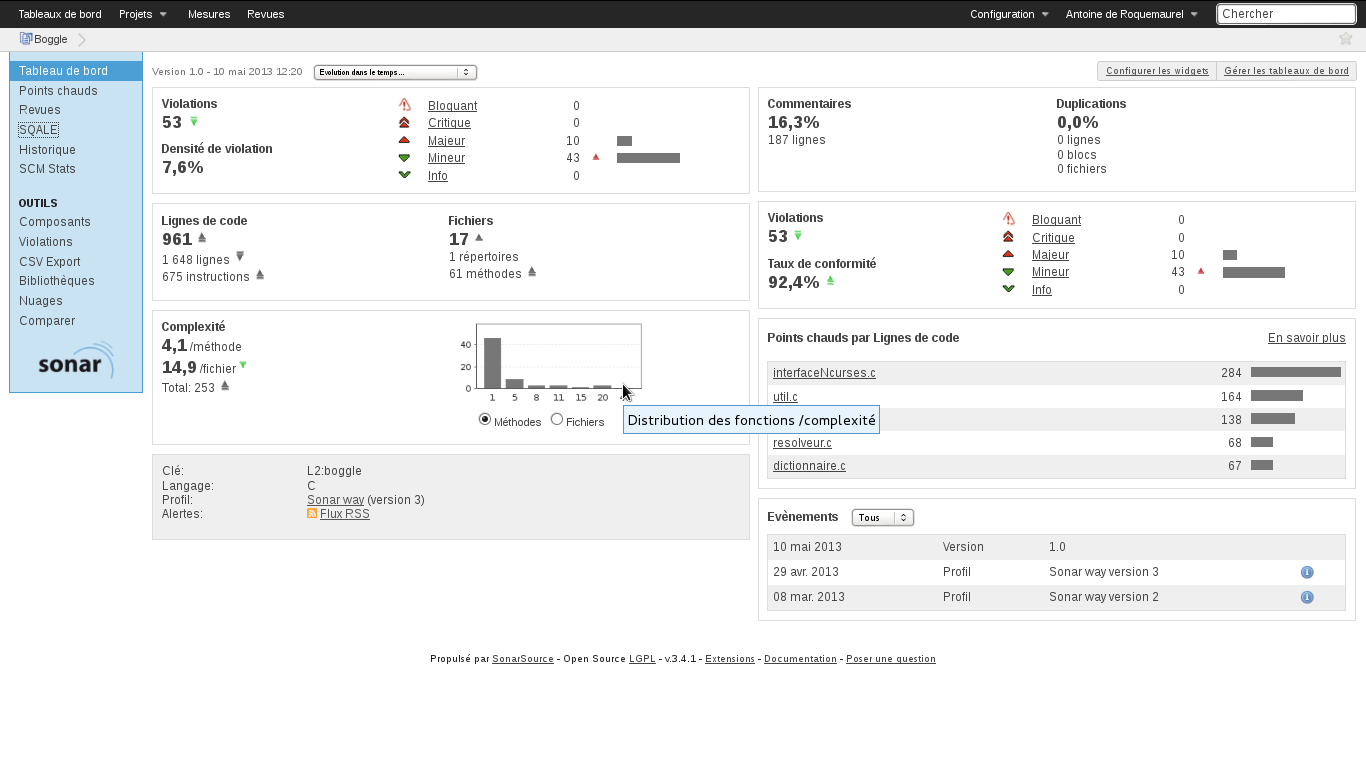
\includegraphics[width=18cm]{screens/sonar.png}
		\caption{Affichage du tableau de bord de \textit{Sonar}}
		\label{fig:sonar}
	\end{figure}
	Sur la figure \ref{fig:sonar}, nous pouvons observer le nombre de ligne effective du programme (nombres de lignes sans compter
	les commentaires), le nombre de fichiers, la complexité par fonction/fichier, la duplication de code, les violations par rapport aux règles de Sonar. 

	\chapter{Tests}
	\chapter{Gestion de projet}
	% TODO blabla bla intro
	Pour ce projet, nous étions deux à travailler dessus, ainsi nous avons utilisé plusieurs techniques afin de se coordonner et de limiter les problèmes. Ceci n'est pas notre premier projet ensemble, notre travail en fut simplifié.
	\section{Un outil de gestion de projet : \textit{Redmine}}
	Pour le projet, nous avons utiliser \textit{Redmine}, une plateforme web de gestion de projet (Cf figure \ref{fig:redmine}). Elle nous a permis de simplifier le travail, et de ne rien oublier.
	En effet, nous pouvons créer des tâches, signaler qu'elles sont en cours/terminés/en tests, leur donner des dates limites, les affecter à une personne etc\ldots
	Ainsi lorsque l'un de nous commençait une tâche, il le signalait sur le \textit{redmine}, ce qui permettait de tenir au courant son binôme de ses actions et
	de l'avancée du projet.
	\begin{figure}[H]
		\centering
		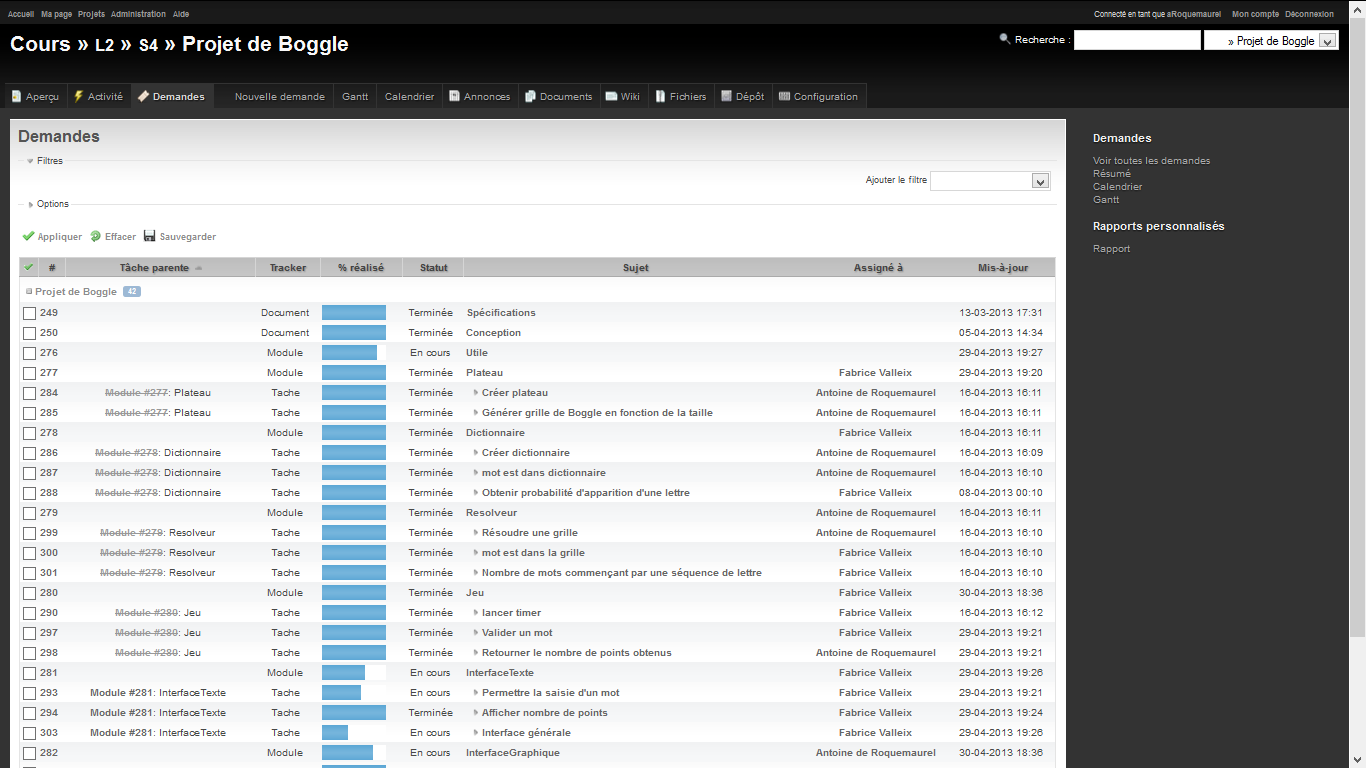
\includegraphics[width=18cm]{screens/redmine.png}
		\caption{Affichage des demandes dans \textit{Redmine}}
		\label{fig:redmine}
	\end{figure}
	Comme le montre la figure \ref{fig:redmine}, nous avons la possibilité de lister toutes les tâches, nous pouvons voir à qui
	elles sont assignées, leurs dates limites, leur hiérarchie etc\ldots

	\textit{Redmine} génère également un diagramme de Gantt,
	nous avons donc utilisé cet utilitaire pour nos
	diagrammes de Gantt\footnote{Disponible en annexe page
	\pageref{gantt}} et
	la liste de nos tâches.

	C'est également sur le wiki de \textit{Redmine} qu'était disponible les conventions d'écritures, mais également des notes sur le
	contrôle de la qualité d'un code, et enfin le fonctionnement de \textit{Git} et \textit{Doxygen}.

	\section{Un logiciel de versionnement : Git}
	Afin de limiter les problèmes du travail collaboratif, nous avons utilisé un logiciel de versionnement Git. Il a deux intérêt, tout d'abord, nous pouvons
	travailler à deux en parallèle sur le projet sans se soucier de fusionner notre travail\footnote{À condition de ne pas travailler sur deux lignes de code identiques}.

	D'autre part, tous les logs étant enregistrés, nous pouvons savoir qui à fait quoi et quel jour, cela permet de voir également l'avancée du projet. 

	Enfin, toutes les modification sont stockées sur le serveur, ainsi en cas de problème, il est très facile de revenir à la version précédente ou même de
	comparer deux versions afin de voir les changements et de comprendre rapidement pourquoi une fonctionnalité a régressé. 
	\appendix
	\chapter{Convention d'écriture en C} \label{conventions}
Voici les conventions écritures que nous avons fixé, il faudra les respecter pour que nous ayons un code propre et homogène, de plus elles ont été fixés pour que ce soit le plus simple pour nous (lecture rapide, propreté etc...)

\section{Le nommage}
\subsection{Les variables globales}
Les variables globales doivent être évitée. Utiliser une variable globale est une abomination, mais si cette utilisation est indisensable, celle-ci doivent être préfixés par g comme ceci.

\begin{lstlisting}[language=C, caption=Exemples de noms de variable globale]
int gMaVariable;
\end{lstlisting}

\subsection{Les variables en paramètre de méthodes}
Les variables paramètre sont les variables qui ne sont que dans une méthode (et donc, elles sont détruites à la fin de la méthode). 
Ces variables doivent respecter la règle précédente à la différences qu'elle doivent toute commencer par un p\_ (pour paramètre)

Ci un paramètre n'est jamais modifié durant la fonction, celui-ci doit être précédé du mot clef const.

\begin{lstlisting}[language=C, caption=Exemples de noms de paramètres]
int pMonSuperParametre;
bool pVousAvezPerdu;
char* pCacamou;
const pMachinChose;
\end{lstlisting}

\subsection{Les noms de constantes ou define}
Les constantes ou \#define doivent être tout en majuscule, les différents mots de la constante sont séparés par des underscore (\_). Même remarque que pour les attributs,
choisissez des noms de constante clair, compréhensible par tous, pas seulement par ceux qui sont dans votre tête! 

Il est préférable d'utiliser des constantes plutôt que des define, celles-ci ayant un typage fort contrairement à ces derniers.

\begin{lstlisting}[language=C, caption=Exemples de noms de constantes]
#define MA_SUPER_CONSTANTE;
#define VOUS_AVEZ_PERDU;
const int CONSTANTE;
\end{lstlisting}

\subsection{Les noms de fonctions}
Les fonctions doivent commencer par une minuscule, et séparer les différents mots par une majuscule. Les fonctions ne retournant rien (procédures) doivent toujours être à l'infinitif. 
À l'opposé les fonctions retournant quelques choses doivent être au participe passé. 
Les fonctions retournant un bouleen doivent être préfixé par le verbe afin d'avoir une lisibilité maximale. estInferieur par exemple
Il faut décomposer au maximum, n'hésitez pas à faire une méthode private si besoin est, c'est toujours plus clair d'avoir une fonction, dictant explicitement ce qu'elle fait par son nom que 10 lignes de code bizarroïdes avec 2-3 lignes de commentaire! Et donc, les noms de fonctions sont essentiels!! 

Chaque noms de fonction doit être préfixé par le nom du module suivis d'un underscore(\_).

Ci une fonction ne contient aucun paramètre, celle-ci doit posséder le paramètre void.
\begin{lstlisting}[language=C, caption=Exemple de fonctions]
void afficher(char* pTexteAAffiche){
    printf("%s", pTexteAAffiche);
}
bool estInferieur(int entier1, int entier2){
   return (entier1 < entier2);
}
void afficherTexte(void){
   printf("coucou");
}
\end{lstlisting}

\subsection{Les noms de type}
Les noms de type doivent tous commencer par une majuscule, les différents mots sont séparés par une majuscule, choisissez des noms de types claires! 
(oui, je me répète, mais c'est ce qui fait toute la compréhension facile, ou non, d'un programme les noms de variables, classe, types, paramètre, méthodes etc... )

\begin{lstlisting}[language=C]
typedef struct {
   int uneVariable;
   char* uneAutreVariable;
} MonSuperType;
\end{lstlisting}

\section{L'indentation}
La règle est simple, on ouvre une accolade, la ligne suivante sera décalé vers la droite(une tab = 4 caractères), on ferme une accolade, on décale l'accolade vers la gauche et tout ce qui suis. 
Egalement, si une ligne est trop longue, on va a la ligne, et décalons d'une ligne vers la droite, une fois l'instruction finie, on redécale vers la gauche.
Dans le cas d'un switch, le break doit s'aligner avec le case 42: tout ce qui est entre case et break sera indenté. 

\begin{lstlisting}[language=C, caption=Exemple d'indentation]
void afficherHelloWorld(){
    printf("Hello World");
    switch(yatta){
        case 42:
            // ^^
        break;
        case 1337:
            // ...
        break;
        default: 
            //
    }
}
}\end{lstlisting}

\section{Les accolades}
Les accolades ouvrante sont positionnés à la fin de la ligne demandant une accolade (switch, if, class, else, elseif, ...)
Les accolades fermantes sont positionnés une ligne après la dernière instruction. (avec une désindentation)
Les else et elseif se mettent sur la même ligne que l'accolades fermante. 

\begin{lstlisting}[language=C, caption=Exemple d'indentation]
    if(true){
        // bla bla
    } else if(false){
        // bla bla 
    } else {
        //instruction
    } 

    switch(var}{
        case 0:
            // ^^
        break;
        case 1:
           // yatta
        break;
        default:
            // :-)
    }
} \end{lstlisting}

	\label{gantt}
	\addcontentsline{toc}{chapter}{B~~Diagramme de Gantt}
	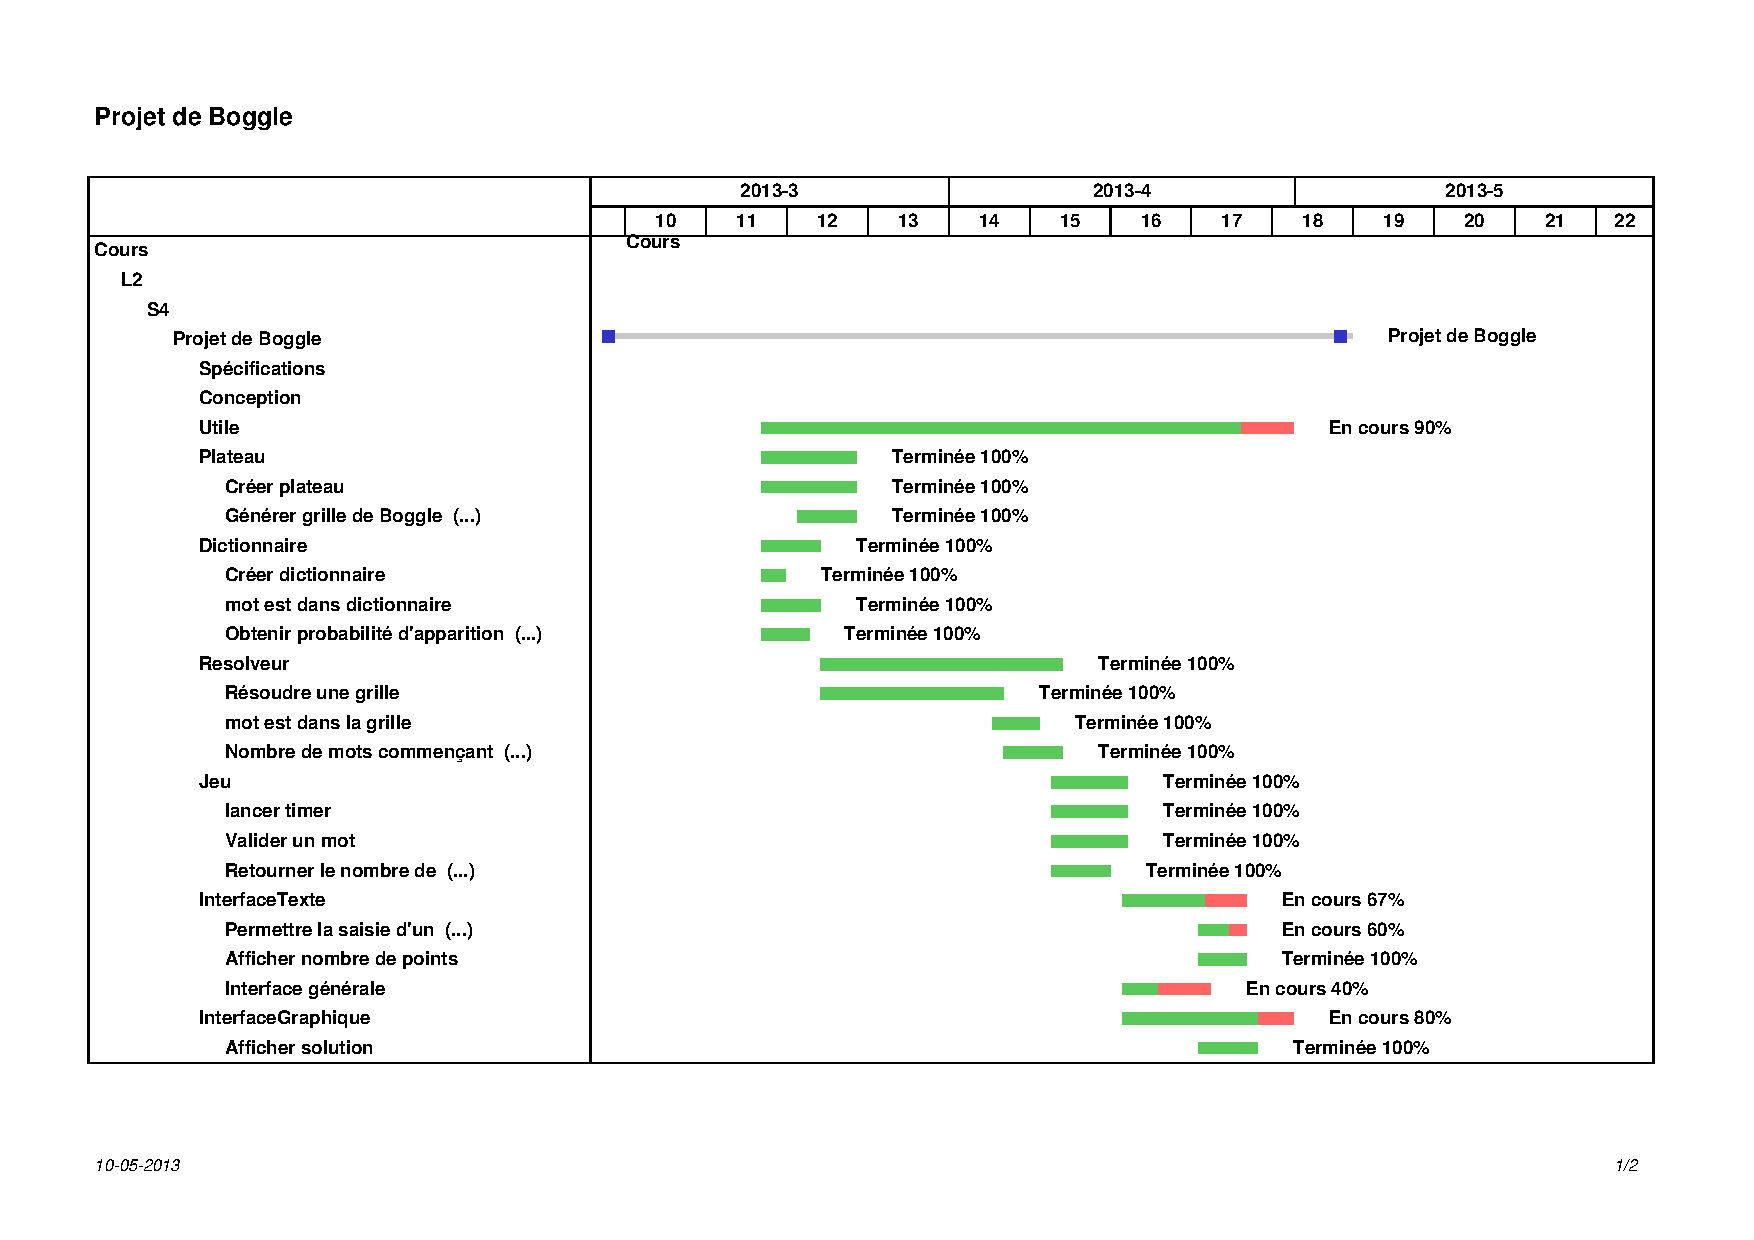
\includepdf[landscape, pages=1-2]{boggle-gantt.pdf}
	\label{conception}
	\addcontentsline{toc}{chapter}{C~~Dossier de conception (Mis à jour)}
	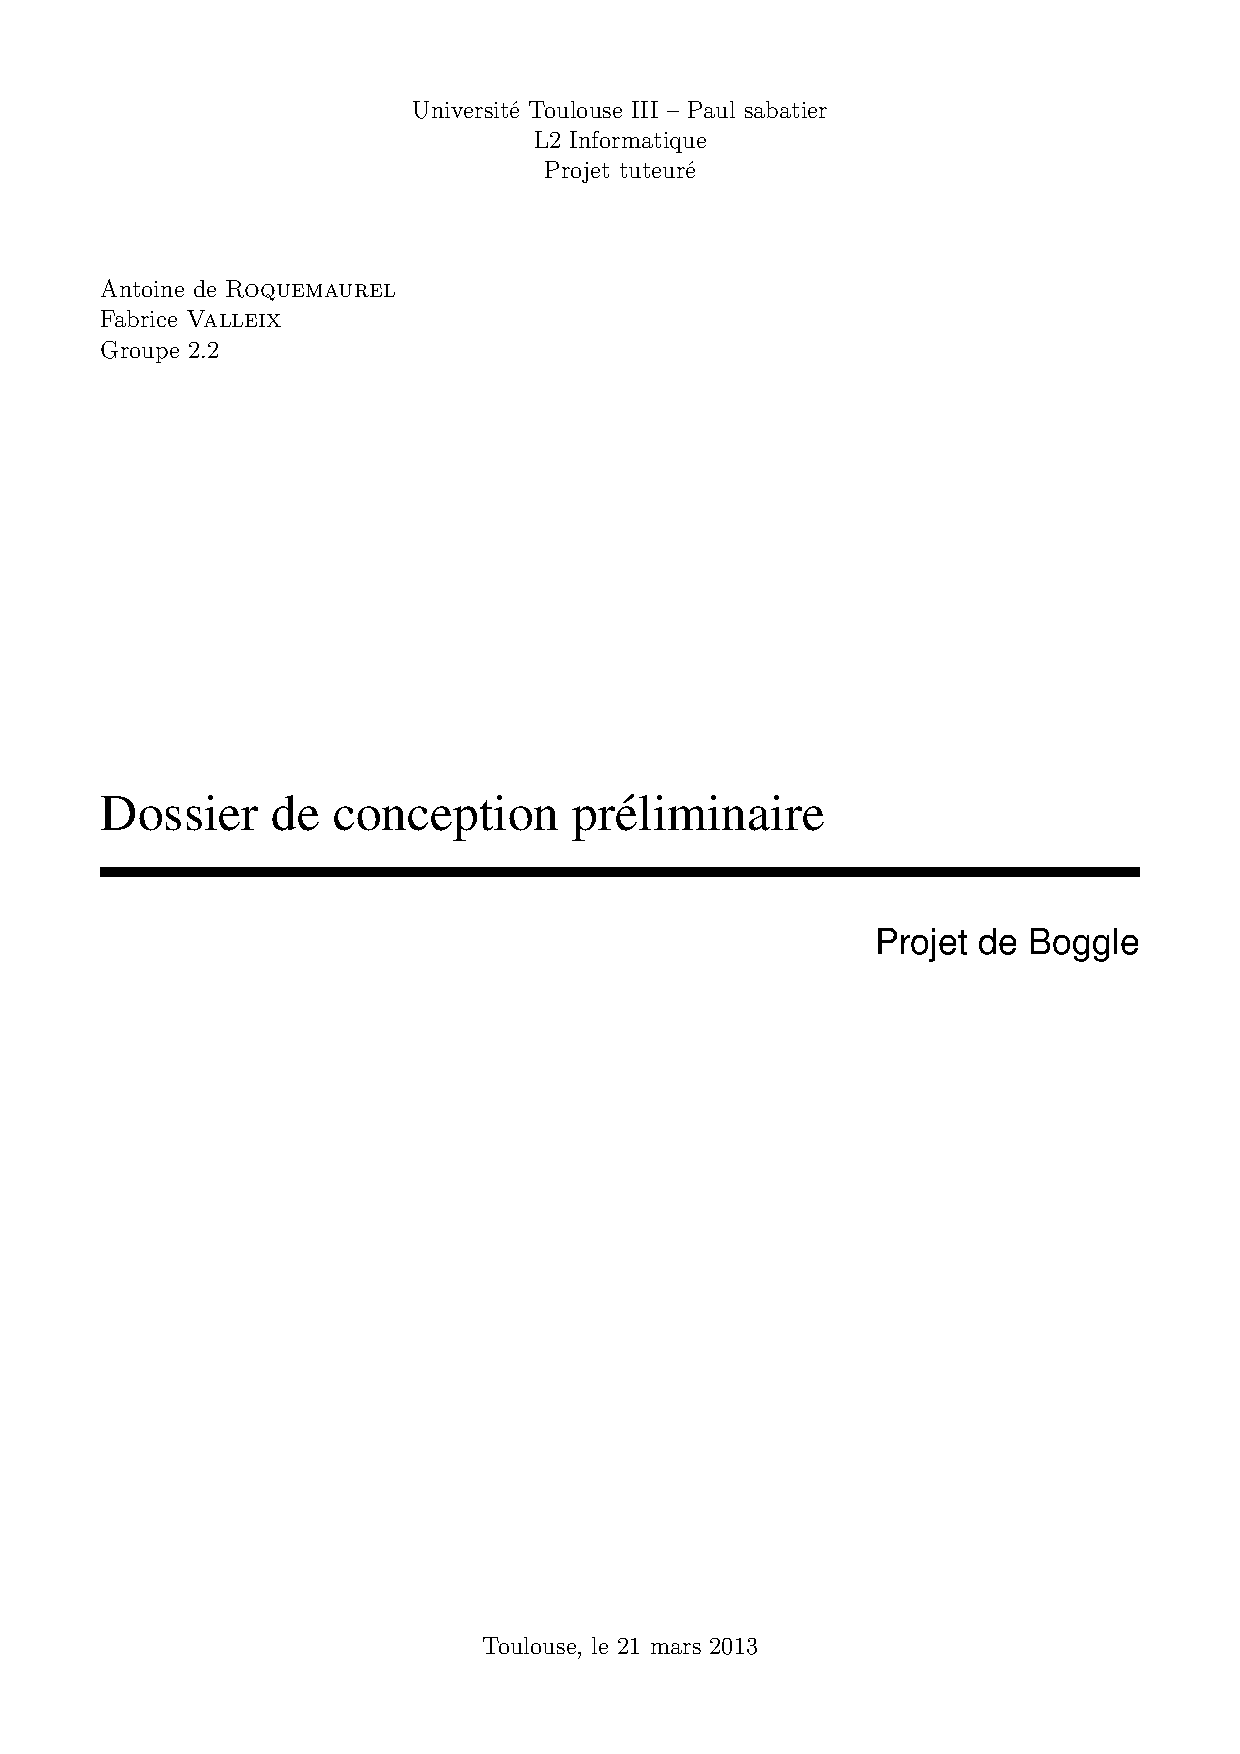
\includepdf[pages=1-]{conception.pdf} %TODO
\end{document}
